\documentclass[11pt, a4paper,twocolumn]{jarticle}
\usepackage[dvipdfmx]{graphicx}
\usepackage{docmute}
\begin{document}
\begin{titlepage}
  \begin{center}
    {\Huge 基礎エレクトロニクス}\\
    \vspace{10truept}
    {\Huge Basic Electoronics}\\
    \vspace{30truept}
    {\huge 提出者 : 08A17153 羽田充宏}\\ % 学籍番号
    \vspace{50truept}

    \begin{list}{}{\setlength{\leftmargin}{95pt}}
    \item {\huge 実験実施日 : 2019年5月13日}\\
    \vspace{10truept}
    \item {\huge 実験実施日 : 2019年5月17日}\\
    \vspace{10truept}
    \item {\huge 実験実施日 : 2019年5月20日}\\
    \vspace{10truept}
    \item {\huge 実験実施日 : 2019年5月24日}\\
    \vspace{10truept}
    \item {\huge 実験実施日 : 2019年5月27日}\\
    \vspace{10truept}
    \item {\huge 実験実施日 : 2019年5月31日}\\
    \vspace{40truept}

    \end{list}
    \vspace{50truept}

  \end{center}
\end{titlepage}


% template======================================================
% \section{}
% \subsection{}
% \subsubsection{Purpose}
% \subsection{Equipment}
% \begin{itemize}
%     \item
% \end{itemize}
% \subsubsection{Procedure}
% \subsubsection{Result}
% \subsubsection{Discussion}
%=============================================================
% \begin{figure}[ht]
%  \begin{center}
%   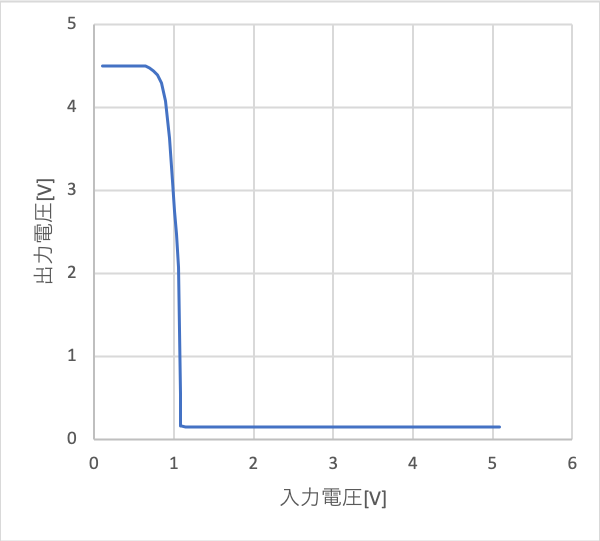
\includegraphics[width=0.8\linewidth]{fig1.png}
%  \end{center}
%  \caption{74HC14}
%  \label{fig:1}
% \end{figure}
% \clearpage
%=============================================================
\twocolumn
[
\begin{center}
    \textbf{\Large Introduction}\\
    \begin{flushleft}
        この実験では電気回路の取り扱いや考え方ついて学ぶ。
        電気回路を応用物理学実験として学ぶ理由には以下のことが挙げられる。
    \end{flushleft}
    \begin{itemize}
        \item 物理学実験において電気回路は重要な役割を果たし,システムの安定性判定や信号増幅の際に必要となるため.
        \item 電気回路を通して様々な物理法則に触れることができる.
        \item 電気回路の中に用いられている半導体は物性物理学のもっとも偉大な発明の一つであり,電気回路を製作する中でどのように半導体が働くかを確認することができる.
        \item デジタル回路はコンピューターアーキテクチャの根幹であるので回路を理解するととはコンピュータテクノロジーを理解することに通じるため.
    \end{itemize}
\end{center}
\vspace{30truept}
]
%=============================================================
\documentclass[11pt, a4paper,twocolumn]{jarticle}
\usepackage[dvipdfmx]{graphicx}
\begin{document}
%=============================================================
\section{光学系の構築 (1日目)}
\subsection{実験目的}
今回の実験目的は光学系のアライメントを正確に行うことと,構築した光学系を用いてビーズのトラッピングを行うことである.

\subsection{実験手順}
まずダイヤルを回して出力電流を変えることでレーザー光の強さを調節した.
次にミラーを2枚用いてレーザー光を光学顕微鏡へ導入し,顕微鏡後側と対物レンズリボルバーに貼り付けられた的の真ん中にレーザー光が通過するようにミラーの位置と角度を調節した.
次にステージにスライドガラスを置いた後,リボルバーに水浸対物レンズを装着し,その上に蒸留水を2滴垂らした.またこのとき補正環は0.17に設定した.
さらに顕微鏡に入射した光がダイクロイックミラーによって試料ステージに反射されるように設定した.
その後CCDカメラによってレーザーがスライドガラス上に集光されることを確認した.
同心円状に集光できているかを確認し,モニターで映し出される集光スポットの中心にシールで目印を付けた.
次にミラーと顕微鏡の間にビームエキスパンダーを挿入し,同心円状に集光するまでビームエキスパンダーの位置の調整を行った.
完成した光学系は図\ref{fig:1}のようになった.

\begin{figure}[htbp]
 \begin{center}
  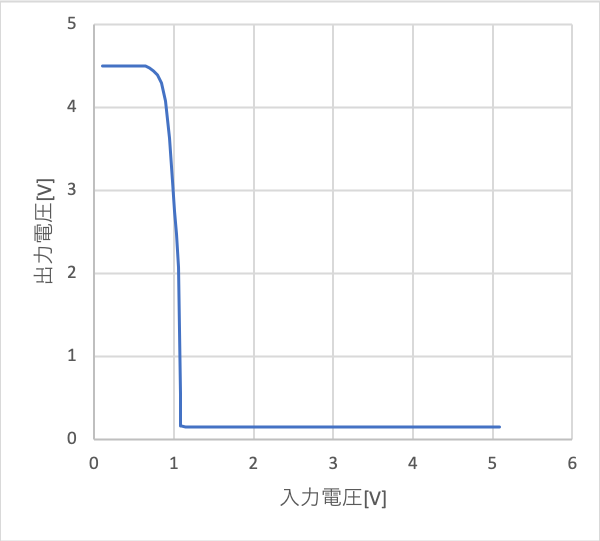
\includegraphics[width=0.8\linewidth]{fig1.png}
 \end{center}
 \caption{実験の光学系}
 \label{fig:1}
\end{figure}

\begin{figure}[htbp]
 \begin{center}
  \includegraphics[width=0.8\linewidth]{fig1-1.png}
 \end{center}
 \caption{同心円状パターン}
 \label{fig:1-1}
\end{figure}

\subsection{結果}
光学系の調整を行った図\ref{fig:1-1}のような同心円状の集光パターンが得られた.
また対物レンズの位置をスライドガラスを置いた試料ステージに近づけていくと2箇所で集光した.



\subsection{考察}
まずビームエキスパンダーを設置した理由について考察する.
レザー光は凸レンズに入射する事で一点に集光するがある程度の広がりを持つ.この時のスポット径を$d_0$,レンズの焦点距離f,レーザー波長$\lambda$,開口の直径をD,媒質の屈折率をnとすると以下の式で表せる.
\begin{equation}
    d = \frac{1.22f\lambda}{nD}
\end{equation}
よってビームエキスパンダーによってDの値を大きくする事でより集光スポットを小さくする目的があると考えられる.

さらに水侵対物レンズを用いる理由は対物レンズを抜けた光が進む媒質を水(n=1.33)にすることで集光スポット径をさらに小さくするためだと考えられる.

顕微鏡に入射した光をダイクロイックミラーで反射させたのは,ダイクロイックミラーが523nm以下の波長の光を透過して,それ以上の波長の光を反射させる性質を利用して,スライドガラスに反射したレザー光によって試料が観測できなくなる事を防ぐ目的であると考えられる.

また,光学顕微鏡へレーザー光を導入するときにミラーを2枚使った理由は任意の座標に任意の方向から光を入射させるためにはミラーが2枚必要であるからだと考えられる.

集光した際に図\ref{fig:1-1}のような同心円状パターンが得られた理由は対物レンズで集光した際にレンズの外側を通過する光と内側を通過する光で光路差が異なるために干渉をおこしレンズ中心からの距離に応じて明線,暗線が生じたためだと考えられる.

%=============================================================
\newpage
\end{document}

\documentclass[11pt, a4paper,twocolumn]{jarticle}
\usepackage[dvipdfmx]{graphicx}
\usepackage{listings,jlisting}

\begin{document}
%=============================================================
\section{Measure of the resistivity($2^{nd} day$)}

\subsection{Purpose}
金属の電流電圧特性を測定する.
\subsection{Procedure}
4端子測定法により以下に示す試料の抵抗を求める.
測定した抵抗値から試料の長さ,直径を考慮してそれぞれの試料の抵抗率を求める.
また今回の測定は全てl = 1cmの幅で行った.
\begin{itemize}
    \item A copper wire
    \item A NiCr wire
    \item A tungsten wire
    \item A lead of automatic pencil(H,2B)
    \item A Ni wire
    \item An Ag wire
    \item An unknown sample
\end{itemize}
\subsection{Result}
測定の結果電流電圧の関係をプロットすると以下のようなグラフが得られた.

\begin{figure}[htbp]
 \begin{center}
  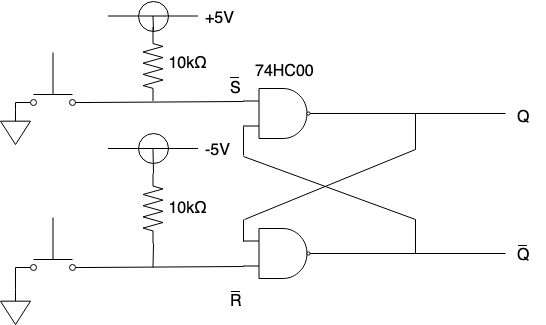
\includegraphics[width=0.8\linewidth]{fig15.png}
 \end{center}
 \caption{Cu}
 \label{fig:15}
\end{figure}

\begin{figure}[htbp]
 \begin{center}
  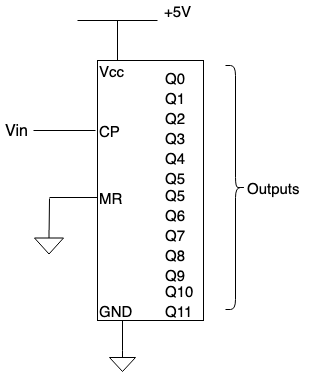
\includegraphics[width=0.8\linewidth]{fig16.png}
 \end{center}
 \caption{NiCr}
 \label{fig:16}
\end{figure}

\begin{figure}[htbp]
 \begin{center}
  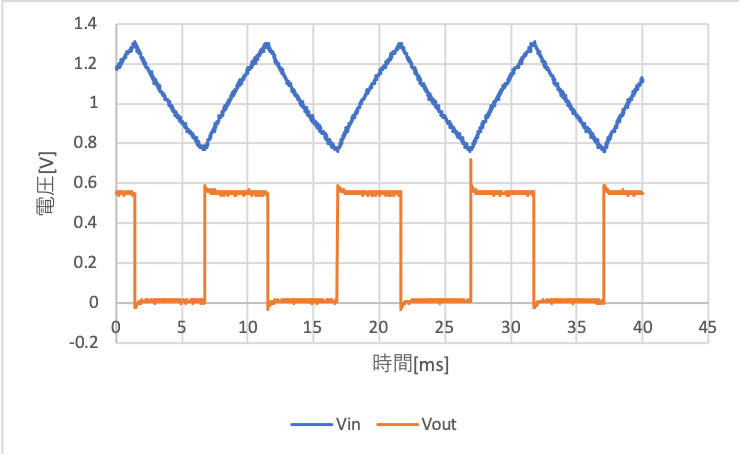
\includegraphics[width=0.8\linewidth]{fig17.png}
 \end{center}
 \caption{W}
 \label{fig:17}
\end{figure}

\begin{figure}[htbp]
 \begin{center}
  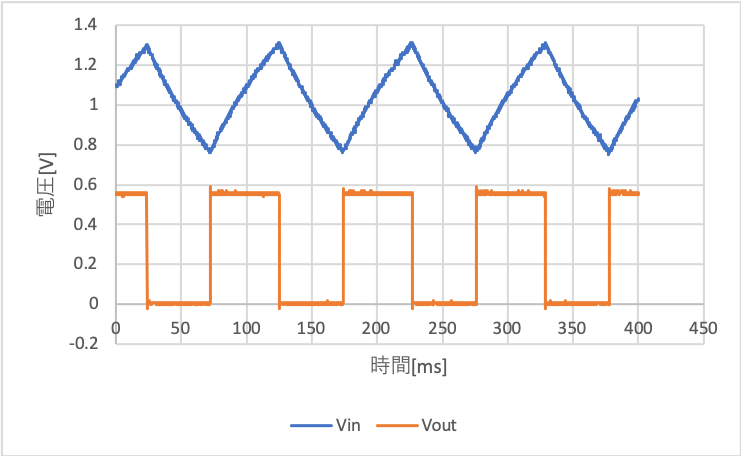
\includegraphics[width=0.8\linewidth]{fig18.png}
 \end{center}
 \caption{シャープペンシルの芯H}
 \label{fig:18}
\end{figure}

\begin{figure}[htbp]
 \begin{center}
  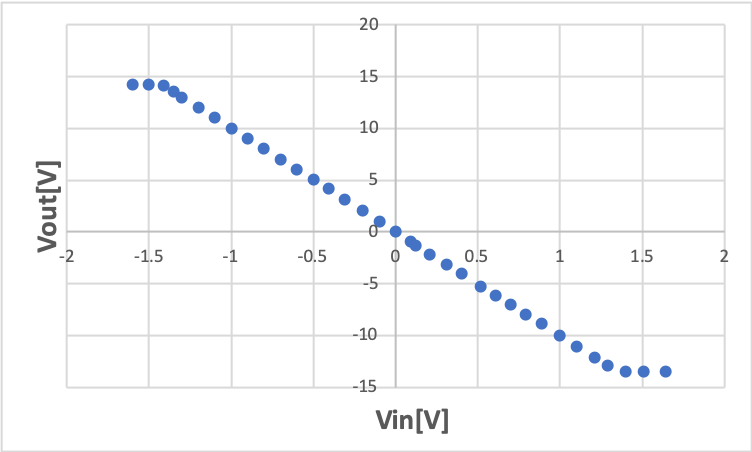
\includegraphics[width=0.8\linewidth]{fig19.png}
 \end{center}
 \caption{シャープペンシルの芯2B}
 \label{fig:19}
\end{figure}

\begin{figure}[htbp]
 \begin{center}
  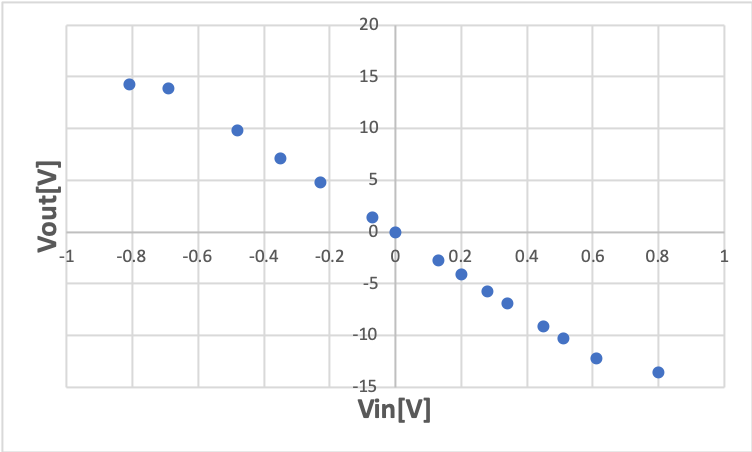
\includegraphics[width=0.8\linewidth]{fig20.png}
 \end{center}
 \caption{Ni}
 \label{fig:20}
\end{figure}

\begin{figure}[htbp]
 \begin{center}
  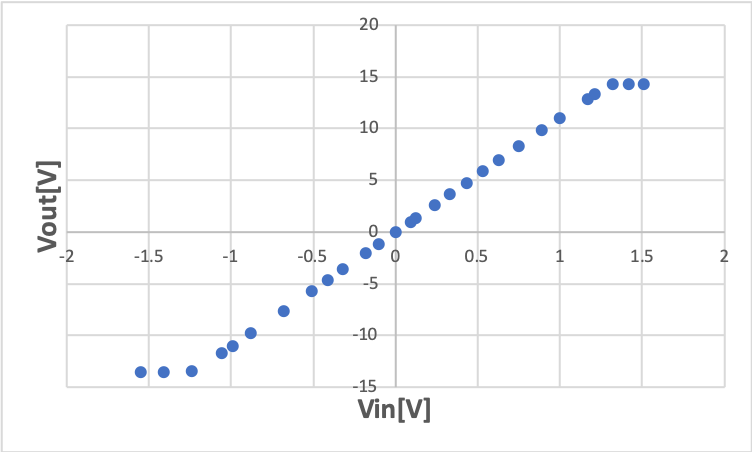
\includegraphics[width=0.8\linewidth]{fig21.png}
 \end{center}
 \caption{Ag}
 \label{fig:21}
\end{figure}

\begin{figure}[htbp]
 \begin{center}
  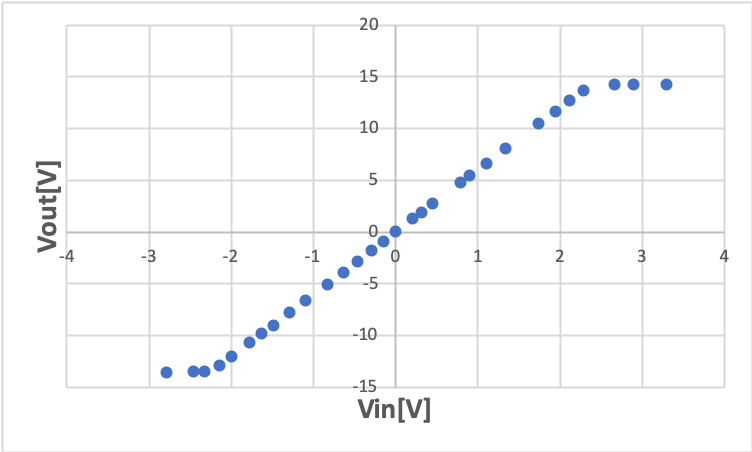
\includegraphics[width=0.8\linewidth]{fig22.png}
 \end{center}
 \caption{不明試料}
 \label{fig:22}
\end{figure}


以上の結果よりグラフの傾きを最小二乗法によって求めそれぞれの抵抗値,抵抗率を求めたところ以下の表のようになった.

\begin{table}[htb]
  \begin{center}
      \caption{抵抗値,抵抗率}
        \begin{tabular}{|c|c|c|} \hline
             試料(直径mm) & 抵抗値($\Omega$) & 2端子($\mu\Omega$cm) \\ \hline
             Cu(0.18) & 0.0132 & 3.35 \\
             NiCr(0.17) & 0.556 & 126 \\
             W(0.09) & 0.1667 & 10.6 \\
             \begin{tabular}{c}
                シャープペンシル \\ の芯H(0.5)
             \end{tabular}
             & 0.3030 & 594 \\
            \begin{tabular}{c}
                シャープペンシル \\ の芯2B(0.5)
            \end{tabular}
             & 0.3030 & 594 \\
             Ni(0.9) & 0.0711 & 45.2 \\
             Ag(0.07) & 0.0386 & 1.49 \\
             不明(0.195) & 0.0735 & 22.0 \\ \hline
        \end{tabular}
  \end{center}
\end{table}

\subsection{Discussion}
どの試料金属においても温度が上昇するにつれて低効率が高くなった現象について考察する.
まず金属はエネルギーバンド図において伝導体に電子を常に持っておりこれは自由電子として電流を運ぶ役割を果たしている.
ここで温度が上昇した場合は格子が熱でより激しく振動することになると予想される.
したがって電子の通り道を格子が塞ぐ確率が高まり結果として単位時間に電子が衝突する回数が多くなり抵抗率が温度の上昇とともに上昇していくと考えられる.
またこの現象から,電子の量が多くなることにより格子に衝突する電子の量が多くなることが予測される.
これはオームの法則の説明であると考えられる.

また測定結果より未知試料だと思われる物質はストロンチウムだと考えられる.
しかし他の金属試料において抵抗率のオーダーはあっているもののその値は理科年表の値から多少ずれており測定において接触抵抗などのノイズが入ったことが考えられる.

またシャープペンシルの芯は濃さに寄らず同じ値を示したことから濃さに寄らずに同じ構造をしていることが予想される.またシャープペンシルの芯はグラフェンであり結合に余分な価電子によって電流を通すが自由電子の数は金属に比べ少ないことが結果から考えられる.
%=============================================================
\newpage
\end{document}

\documentclass[11pt, a4paper,twocolumn]{jarticle}
\usepackage[dvipdfmx]{graphicx}
\usepackage{listings,jlisting}

\begin{document}
%=============================================================
\section{To understand the current-voltage characteristic of semiconductor diodes($3^{rd} day$)}

\subsection{Purpose}
半導体の電流電圧特性を理解する.
\subsection{Procedure}
Siベースダイオード,LED,ツェナーダイオードの三種類の資料について電流電圧特性を計測する.
この時電流が40mAを超えないように注意する.
またヒステリシス特性を観察するために電圧を上昇させた場合と下降させて行った場合の2通りを2回ずつ測定した.

\subsection{Result}
測定の結果電流電圧の関係をプロットすると以下のようなグラフが得られた.
グラフよりいずれのダイオードもある一定の電圧がかからなければ電流を通さない性質を示した.

LEDについては電流が流れるのと同時に発光し始め,電圧を高くするにつれて光は強くなっていった.またいずれのダイオードも逆方向に電圧をかけても電流は流れなかった.

さらにグラフよりわかるように電圧をあげていった場合も電圧を下げた場合も電流の値は同じ値を取ったためヒステリシス特性は示さなかった.

\begin{figure}[htbp]
 \begin{center}
  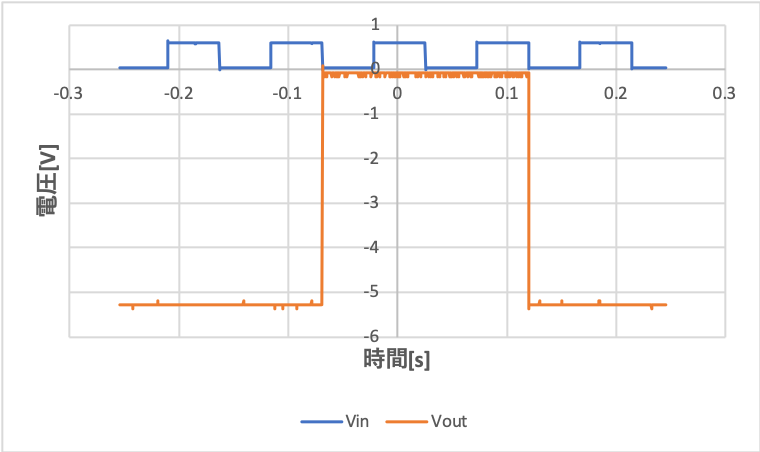
\includegraphics[width=0.8\linewidth]{fig23.png}
 \end{center}
 \caption{LED 1回目}
 \label{fig:23}
\end{figure}

\begin{figure}[htbp]
 \begin{center}
  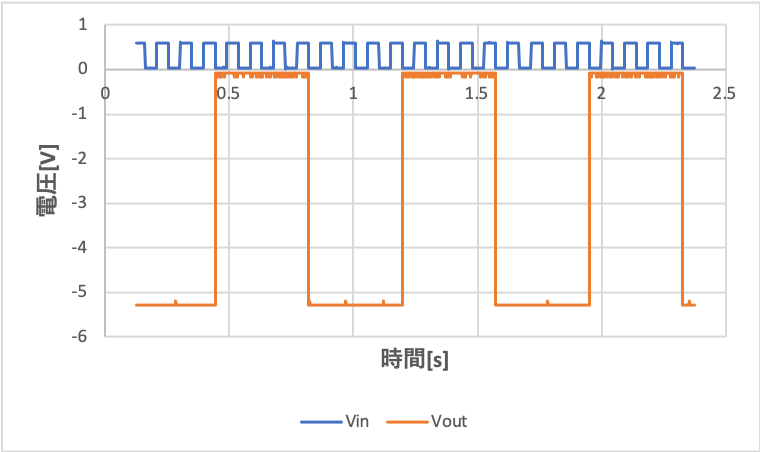
\includegraphics[width=0.8\linewidth]{fig24.png}
 \end{center}
 \caption{LED 2回目}
 \label{fig:24}
\end{figure}

\begin{figure}[htbp]
 \begin{center}
  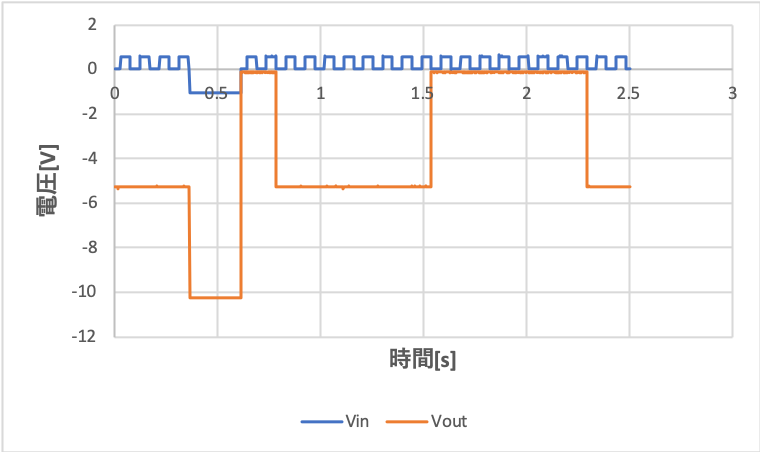
\includegraphics[width=0.8\linewidth]{fig25.png}
 \end{center}
 \caption{Siダイオード 1回目}
 \label{fig:25}
\end{figure}

\begin{figure}[htbp]
 \begin{center}
  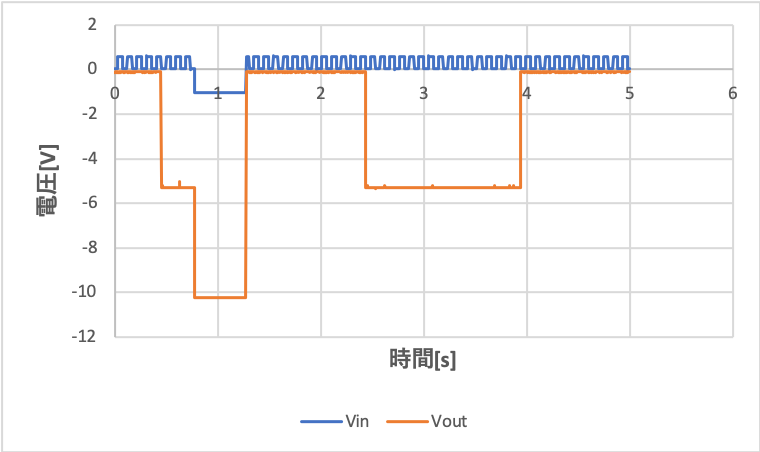
\includegraphics[width=0.8\linewidth]{fig26.png}
 \end{center}
 \caption{Siダイオード 2回目}
 \label{fig:26}
\end{figure}

\newpage

\begin{figure}[htbp]
 \begin{center}
  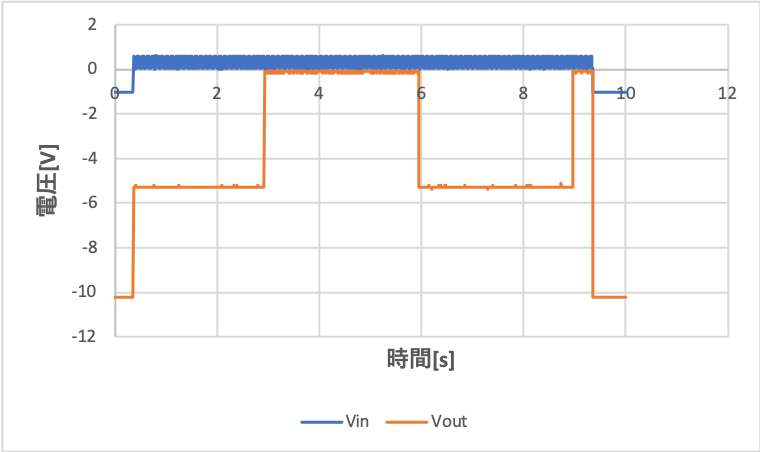
\includegraphics[width=0.8\linewidth]{fig27.png}
 \end{center}
 \caption{ツェナーダイオード 1回目}
 \label{fig:27}
\end{figure}

\begin{figure}[htbp]
 \begin{center}
  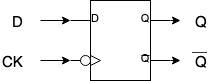
\includegraphics[width=0.8\linewidth]{fig28.png}
 \end{center}
 \caption{ツェナーダイオード 2回目}
 \label{fig:28}
\end{figure}



\subsection{Discussion}
実験結果よりダイオードは順バイアス電圧をかけた際には電流を流すが逆バイアス時には電流は流れない整流作用の特性を持つので電流が逆流して欲しくない回路などに組み込んで応用することができると考えられる.

次にダイオードの順バイアス時にある特定の電圧を超えた際に電流を流し始める特性について考察する.
まずPN接合においては図\ref{fig:36}のようにP領域のキャリアとN領域の電子がそれぞれ接触し消滅する空乏層が生成される.
この空乏層が障壁となるため順バイアスを印加した際にある一定電圧を超えないと電流を流さないのはこの電位障壁が理由だと考えられる.
また逆バイアスをかけた際は空乏層を広げることとなりこの時は電流を流すことはなくなる.これが整流作用の原理だと考えられる.

また逆バイアスをさらに印加していった際の振る舞いについて考察する.
非常に大きな電圧を逆バイアスに印加した際はN型半導体の領域において電子は非常に大きな運動エネルギーを持つことになるがこの運動エネルギーが振動する格子に衝突することで減少し,格子にエネルギーが受け渡されるがこのエネルギーが格子の電子を励起させるのに十分な運動エネルギーを持っていた場合,ぶつかった格子から新たに自由電子とホールのペアが生成される.
またこの反応が再帰的に起こることで急激に電流が流れることが予想される.
今回は実験の時間により逆バイアスの測定ができなかったが図\ref{fig:37}のように電圧電流特性を示すことが予想される.



\begin{figure}[htbp]
 \begin{center}
  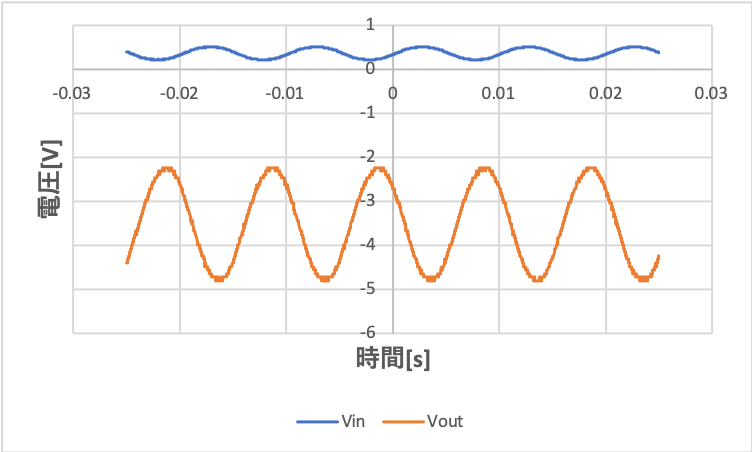
\includegraphics[width=0.8\linewidth]{fig36.png}
 \end{center}
 \caption{PN接合}
 \label{fig:36}
\end{figure}

\begin{figure}[htbp]
 \begin{center}
  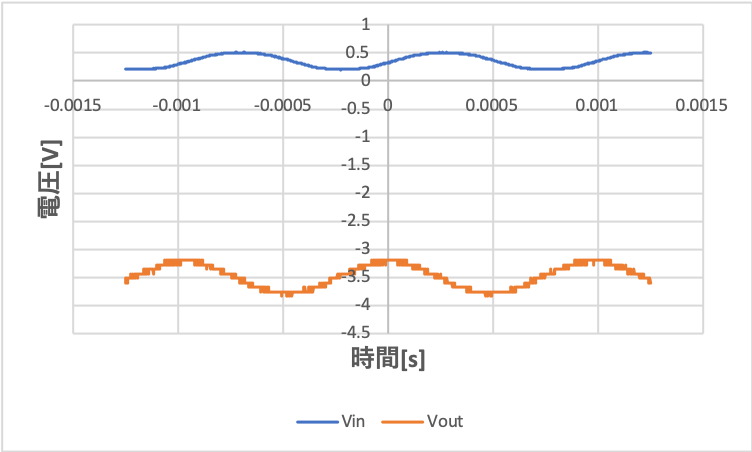
\includegraphics[width=0.8\linewidth]{fig37.png}
 \end{center}
 \caption{電流電圧特性}
 \label{fig:37}
\end{figure}


%=============================================================
\newpage
\end{document}

\documentclass[11pt, a4paper,twocolumn]{jarticle}
\usepackage[dvipdfmx]{graphicx}
\usepackage{docmute}
\begin{document}
%=============================================================
\section{Frequency filters \\based on operational amplifiers ($4^{th} \& 5^{th} day$)}
\subsubsection{Purpose}
増幅器を使いlow-pass filter, high-pass filter 作り,それを用いて周波数時間特性を調べる.
\subsection{Equipment}
\begin{itemize}
    \item 実験3と同様のもの
\end{itemize}
\subsubsection{Procedure}
まず図\ref{fig:12}に示すようにLow-pass-filterを作る.
この時オペアンプのパワーラインとGNDに前回同様0.1$\mu$Fのコンデンサを挟むことを確認する.
今回の実験ではファンクションジェネレーターを用いて矩形波,正弦波を作る.
まず$V_{in}$にファンクションジェネレーターを用いて矩形波を入力とし,10Hzから10KHzまで10倍づつ変化させながら測定した.
この時オシロスコープを用いて矩形波の入力電圧と出力電圧を同時に表示して観察した.
またこの時のデータをUSBに保存した.
次に正弦波を同様の手順で測定し記録した.

次に図\ref{fig:13}に示すようにHigh-pass-filterを作り,前回同様ファンクションジェネレーターにより矩形波の入力電圧と出力電圧の関係を測定し,次に正弦波の入力電圧と出力電圧の関係を測定した.

最後に図\ref{fig:14}に示すようにBand-pass-filterを作り,前回同様に矩形波,正弦波の入力電圧においてそれぞれ周波数を変えながら測定を行なった.

これらの実験から得られた結果を対数グラフにプロットすることによって周波数と振幅の関係について調べる.
また出力電圧の波形と入力電圧の波形を見比べてその位相差について調べる.

\begin{figure}[htbp]
 \begin{center}
  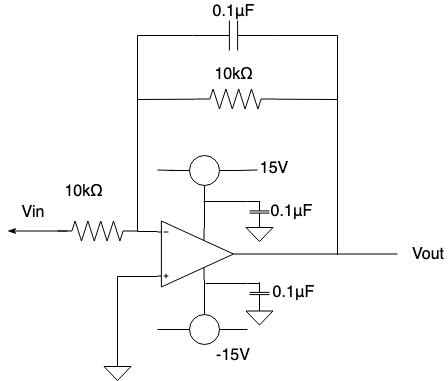
\includegraphics[width=0.8\linewidth]{fig12.png}
 \end{center}
 \caption{High pass filter}
 \label{fig:12}
\end{figure}

\begin{figure}[htbp]
 \begin{center}
  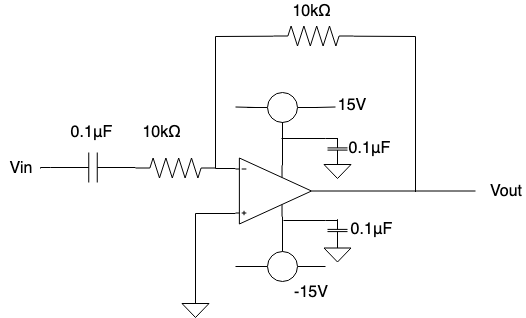
\includegraphics[width=0.8\linewidth]{fig13.png}
 \end{center}
 \caption{Low pass filter}
 \label{fig:13}
\end{figure}

\begin{figure}[htbp]
 \begin{center}
  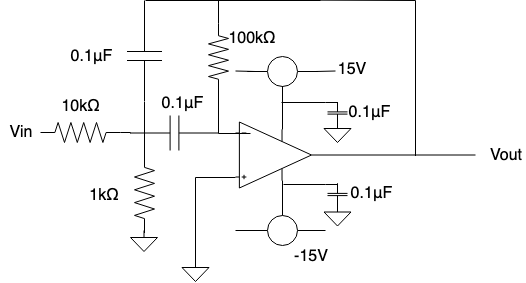
\includegraphics[width=0.8\linewidth]{fig14.png}
 \end{center}
 \caption{Band pass filter}
 \label{fig:14}
\end{figure}

\subsubsection{Result}
測定の結果まず,Low pass filterについて以下のような結果が得られた.
まずは矩形波についての結果をしめす.

\begin{figure}[htbp]
 \begin{center}
  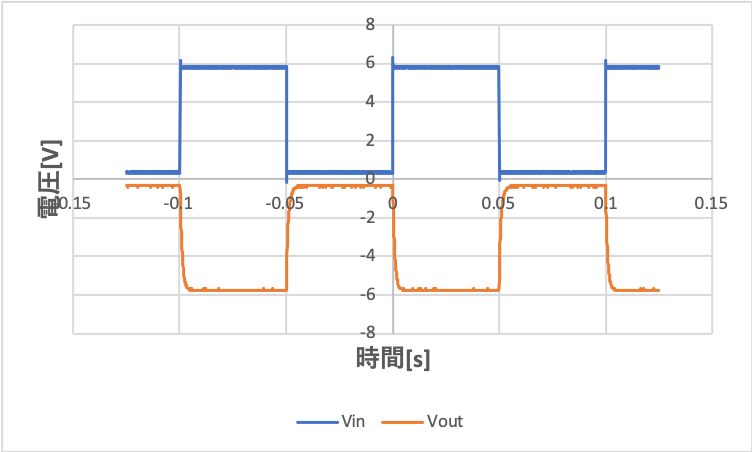
\includegraphics[width=0.8\linewidth]{fig31.png}
 \end{center}
 \caption{Low pass filter(Vin 10Hz)}
 \label{fig:31}
\end{figure}

\begin{figure}[htbp]
 \begin{center}
  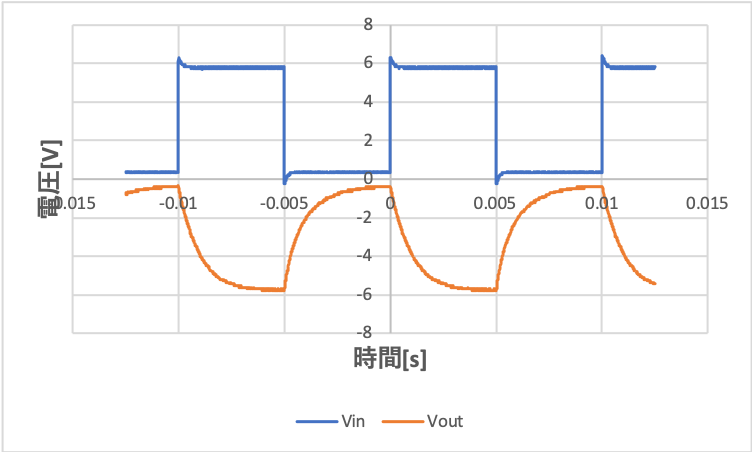
\includegraphics[width=0.8\linewidth]{fig32.png}
 \end{center}
 \caption{Low pass filter(Vin 100Hz)}
 \label{fig:32}
\end{figure}

\begin{figure}[htbp]
 \begin{center}
  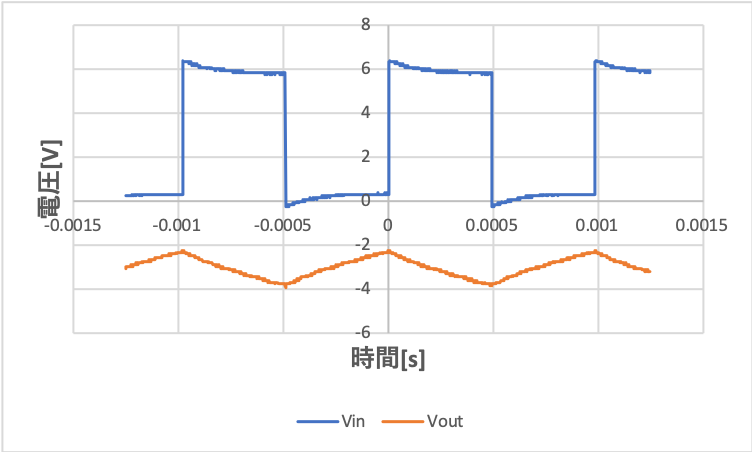
\includegraphics[width=0.8\linewidth]{fig33.png}
 \end{center}
 \caption{Low pass filter(Vin 1kHz)}
 \label{fig:33}
\end{figure}

\begin{figure}[htbp]
 \begin{center}
  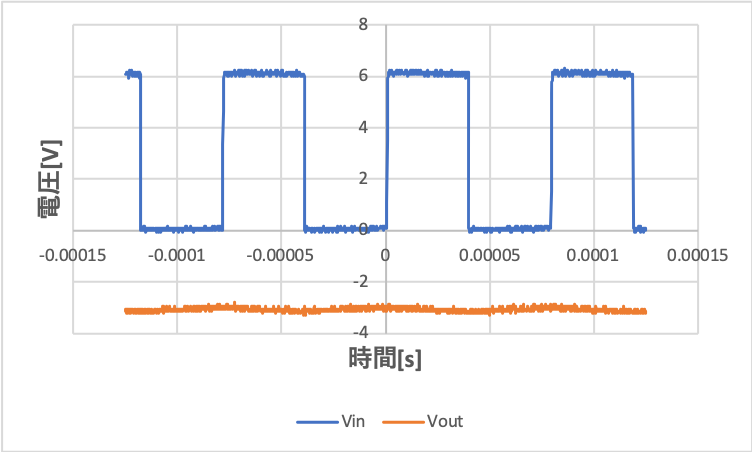
\includegraphics[width=0.8\linewidth]{fig34.png}
 \end{center}
 \caption{Low pass filter(Vin 10kHz)}
 \label{fig:34}
\end{figure}

\newpage

続いて正弦波についての結果を示す.

\begin{figure}[htbp]
 \begin{center}
  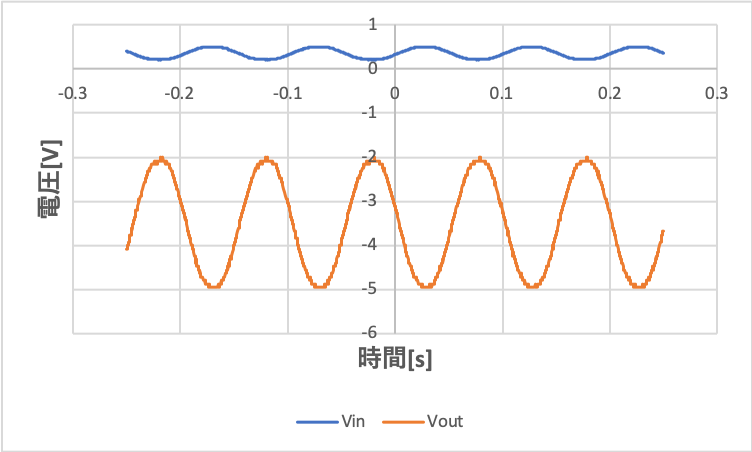
\includegraphics[width=0.8\linewidth]{fig35.png}
 \end{center}
 \caption{Low pass filter(Vin 10Hz)}
 \label{fig:35}
\end{figure}

\begin{figure}[htbp]
 \begin{center}
  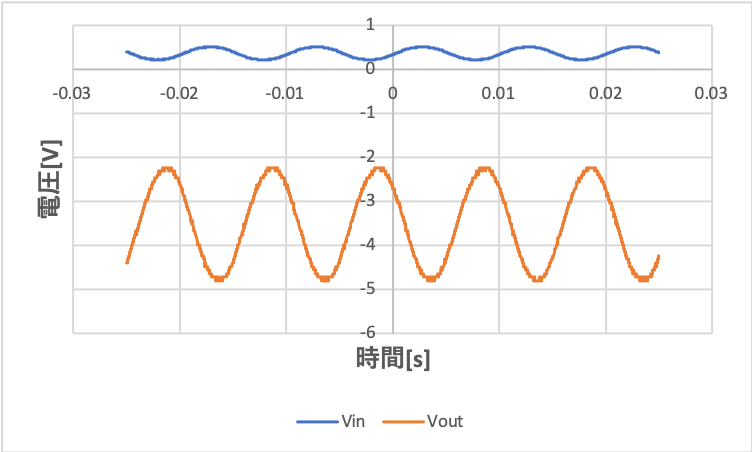
\includegraphics[width=0.8\linewidth]{fig36.png}
 \end{center}
 \caption{Low pass filter(Vin 100Hz)}
 \label{fig:36}
\end{figure}

\begin{figure}[htbp]
 \begin{center}
  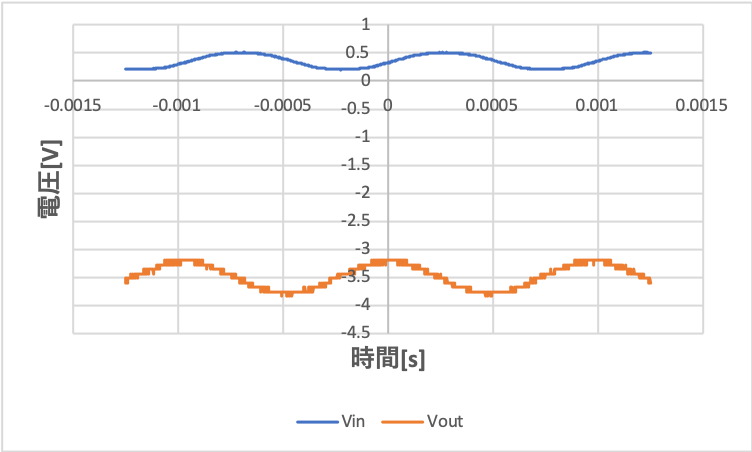
\includegraphics[width=0.8\linewidth]{fig37.png}
 \end{center}
 \caption{Low pass filter(Vin 1kHz)}
 \label{fig:37}
\end{figure}

\begin{figure}[htbp]
 \begin{center}
  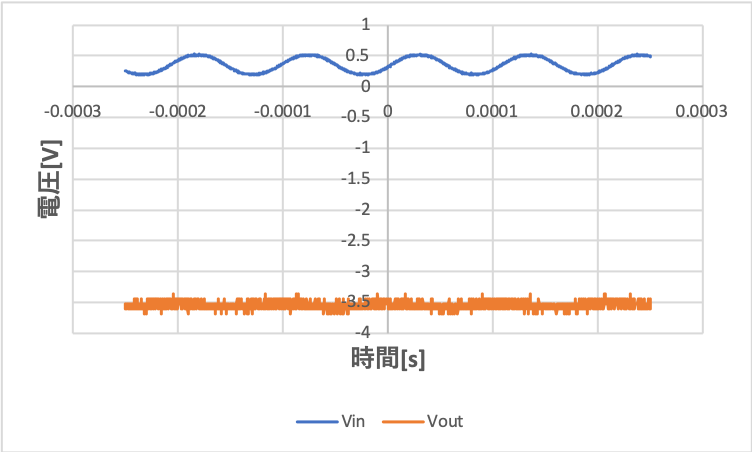
\includegraphics[width=0.8\linewidth]{fig38.png}
 \end{center}
 \caption{Low pass filter(Vin 10kHz)}
 \label{fig:38}
\end{figure}

\newpage

さらにHigh pass filterについても以下のような結果が得られた.
まずは矩形波の結果を示す.

\begin{figure}[htbp]
 \begin{center}
  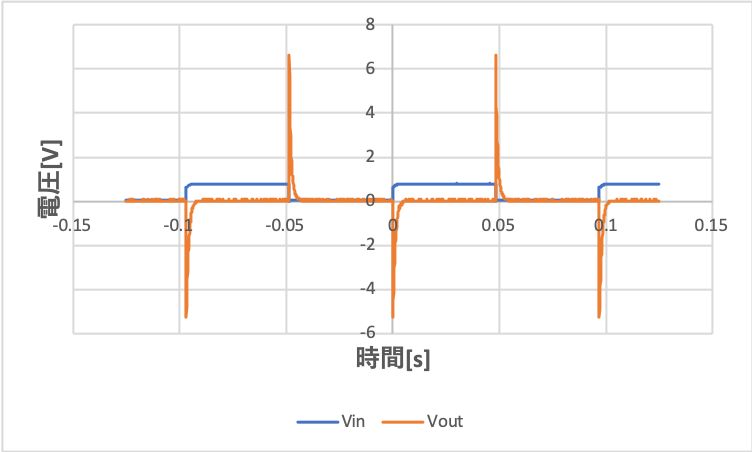
\includegraphics[width=0.8\linewidth]{fig39.png}
 \end{center}
 \caption{High pass filter(Vin 10Hz)}
 \label{fig:39}
\end{figure}

\begin{figure}[htbp]
 \begin{center}
  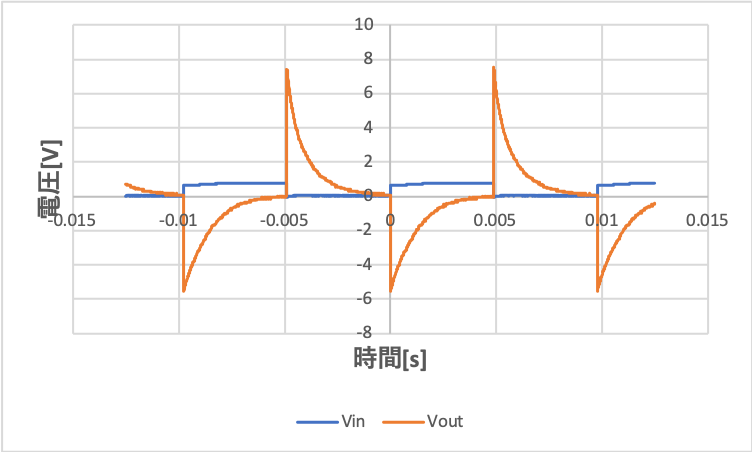
\includegraphics[width=0.8\linewidth]{fig40.png}
 \end{center}
 \caption{High pass filter(Vin 100Hz)}
 \label{fig:40}
\end{figure}

\begin{figure}[htbp]
 \begin{center}
  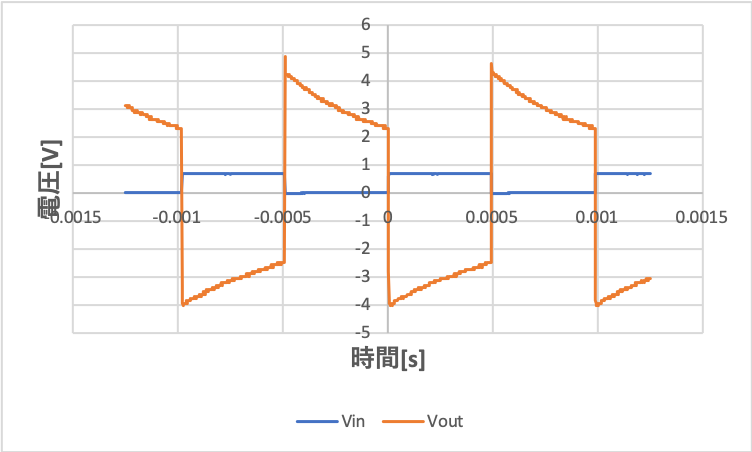
\includegraphics[width=0.8\linewidth]{fig41.png}
 \end{center}
 \caption{High pass filter(Vin 1kHz)}
 \label{fig:41}
\end{figure}

\begin{figure}[htbp]
 \begin{center}
  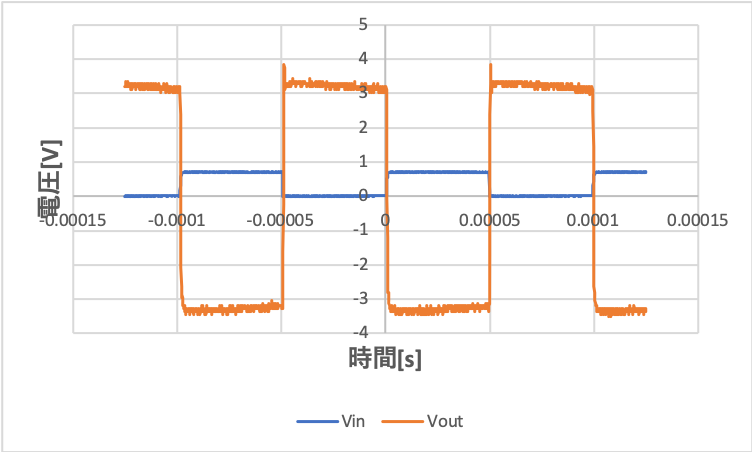
\includegraphics[width=0.8\linewidth]{fig42.png}
 \end{center}
 \caption{High pass filter(Vin 10kHz)}
 \label{fig:42}
\end{figure}

\newpage

続いて正弦波の結果を以下に示す.

\begin{figure}[htbp]
 \begin{center}
  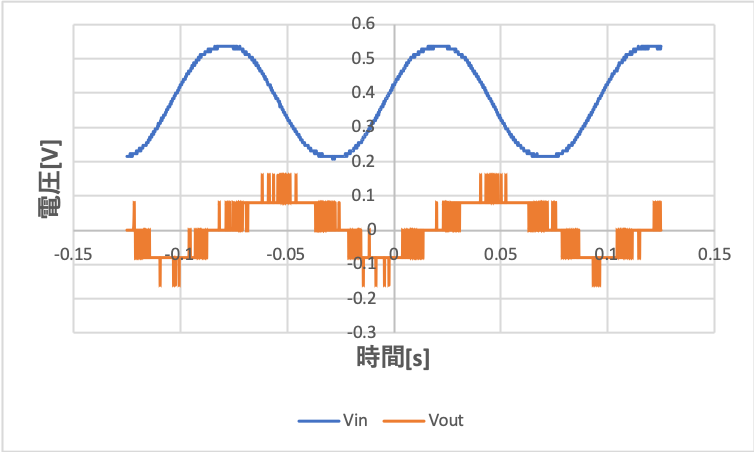
\includegraphics[width=0.8\linewidth]{fig43.png}
 \end{center}
 \caption{High pass filter(Vin 10Hz)}
 \label{fig:43}
\end{figure}

\begin{figure}[htbp]
 \begin{center}
  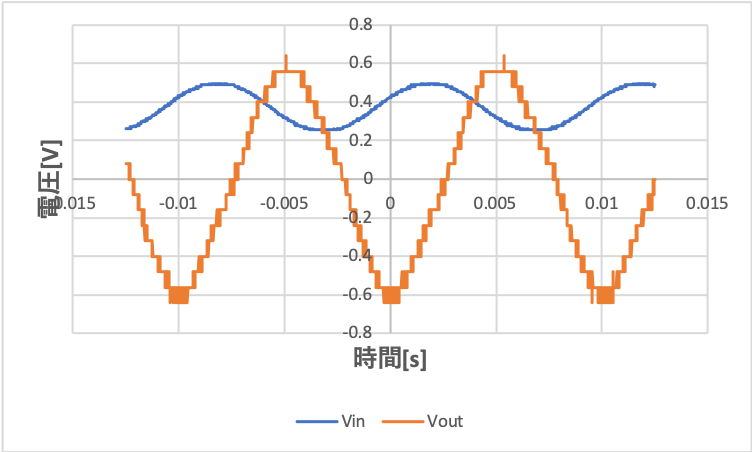
\includegraphics[width=0.8\linewidth]{fig44.png}
 \end{center}
 \caption{High pass filter(Vin 100Hz)}
 \label{fig:44}
\end{figure}

\begin{figure}[htbp]
 \begin{center}
  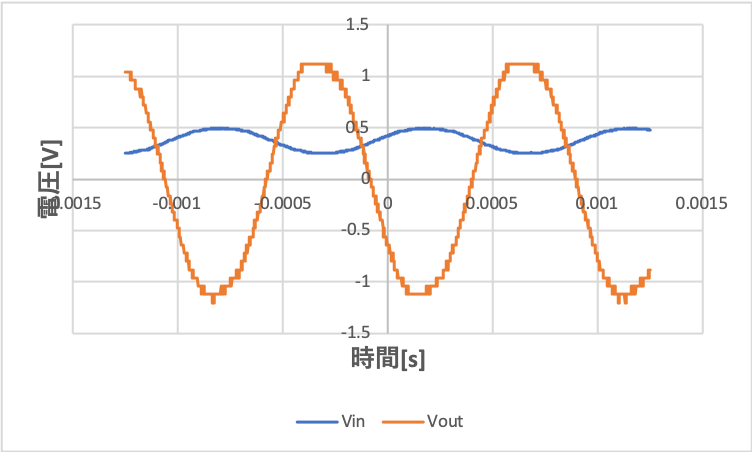
\includegraphics[width=0.8\linewidth]{fig45.png}
 \end{center}
 \caption{High pass filter(Vin 1kHz)}
 \label{fig:45}
\end{figure}

\begin{figure}[htbp]
 \begin{center}
  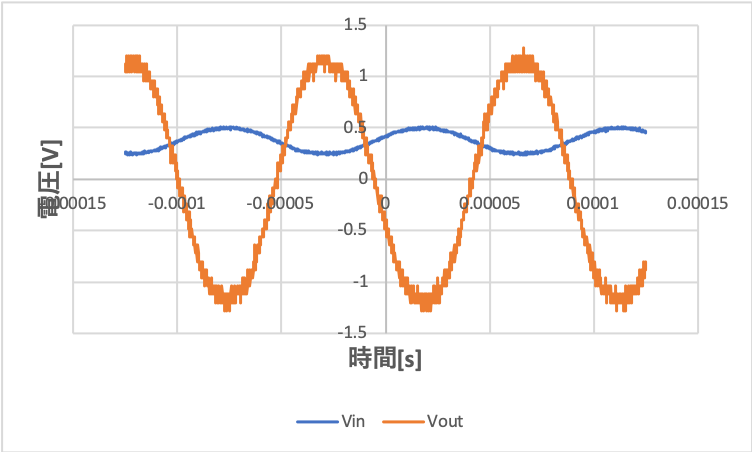
\includegraphics[width=0.8\linewidth]{fig46.png}
 \end{center}
 \caption{High pass filter(Vin 10kHz)}
 \label{fig:46}
\end{figure}

\newpage

最後にBand pass filterについても以下のような結果が得られた.
まずは矩形波の結果を示す.

\begin{figure}[htbp]
 \begin{center}
  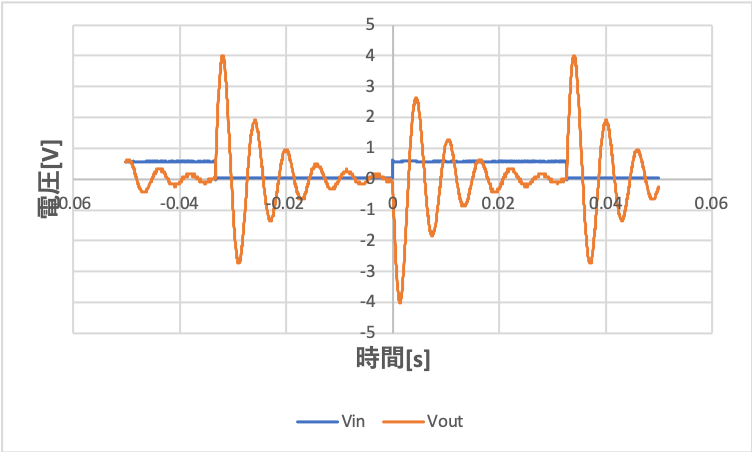
\includegraphics[width=0.8\linewidth]{fig47.png}
 \end{center}
 \caption{Band pass filter(Vin 10Hz)}
 \label{fig:47}
\end{figure}

\begin{figure}[htbp]
 \begin{center}
  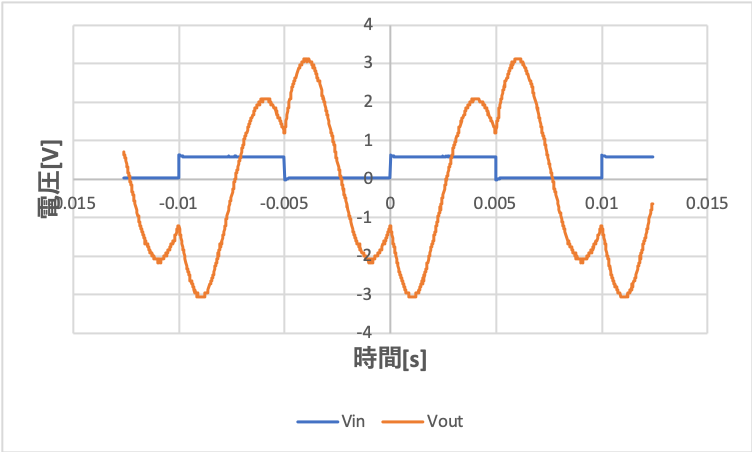
\includegraphics[width=0.8\linewidth]{fig48.png}
 \end{center}
 \caption{Band pass filter(Vin 100Hz)}
 \label{fig:48}
\end{figure}

\begin{figure}[htbp]
 \begin{center}
  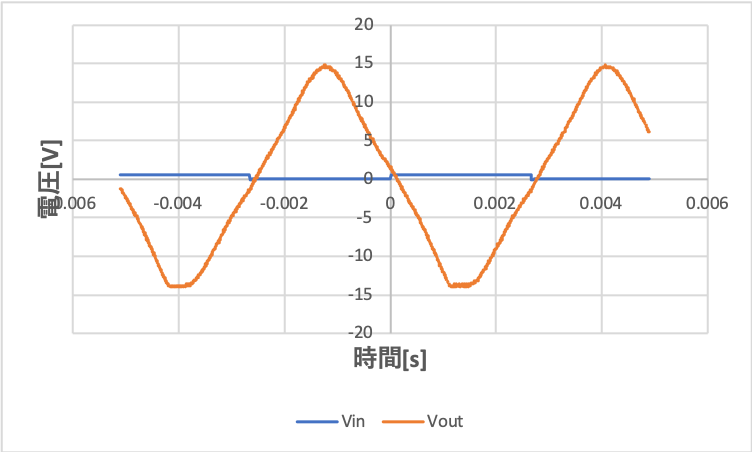
\includegraphics[width=0.8\linewidth]{fig49.png}
 \end{center}
 \caption{Band pass filter(Vin 2kHz)}
 \label{fig:49}
\end{figure}

\begin{figure}[htbp]
 \begin{center}
  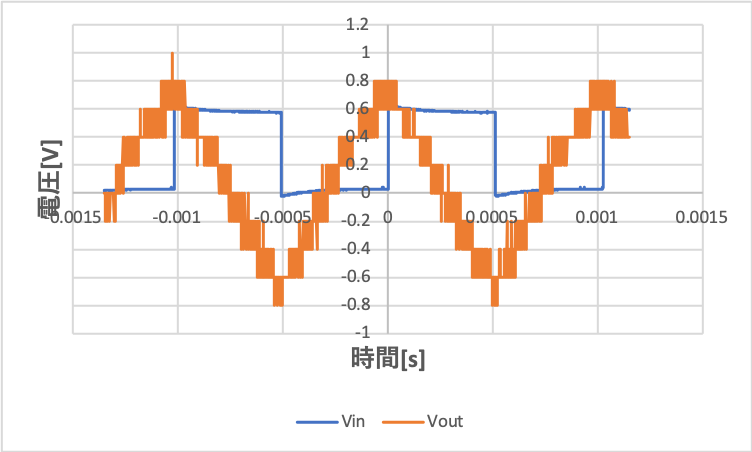
\includegraphics[width=0.8\linewidth]{fig50.png}
 \end{center}
 \caption{Band pass filter(Vin 10kHz)}
 \label{fig:50}
\end{figure}

\newpage

続いて正弦波の結果を以下に示す.

\begin{figure}[htbp]
 \begin{center}
  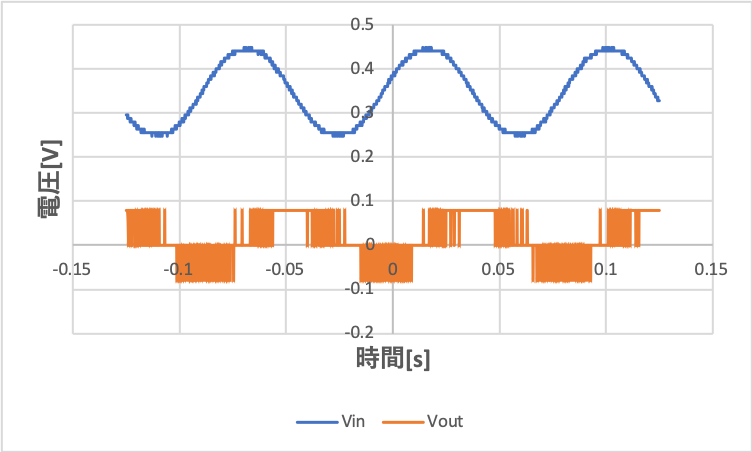
\includegraphics[width=0.8\linewidth]{fig51.png}
 \end{center}
 \caption{Band pass filter(Vin 10Hz)}
 \label{fig:51}
\end{figure}

\begin{figure}[htbp]
 \begin{center}
  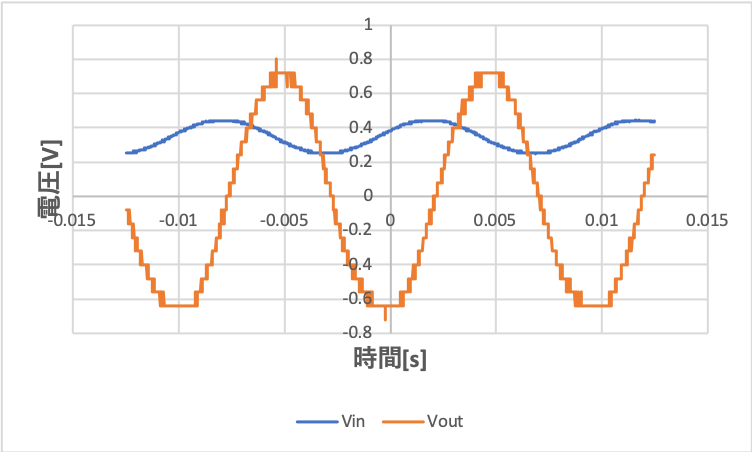
\includegraphics[width=0.8\linewidth]{fig52.png}
 \end{center}
 \caption{Band pass filter(Vin 100Hz)}
 \label{fig:52}
\end{figure}

\begin{figure}[htbp]
 \begin{center}
  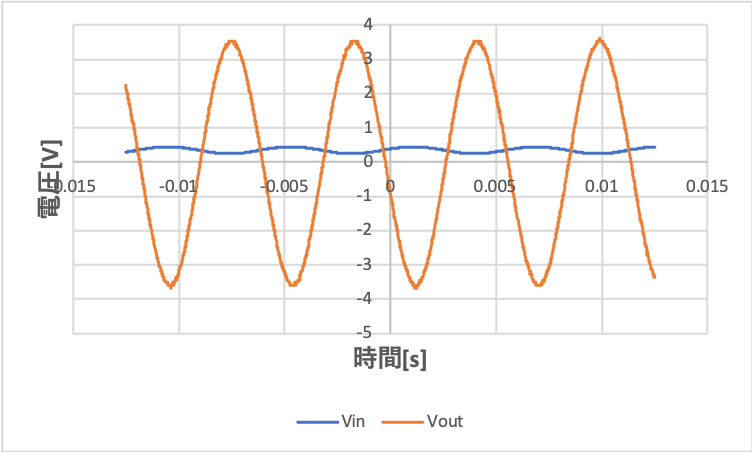
\includegraphics[width=0.8\linewidth]{fig53.png}
 \end{center}
 \caption{Band pass filter(Vin 1kHz)}
 \label{fig:53}
\end{figure}

\begin{figure}[htbp]
 \begin{center}
  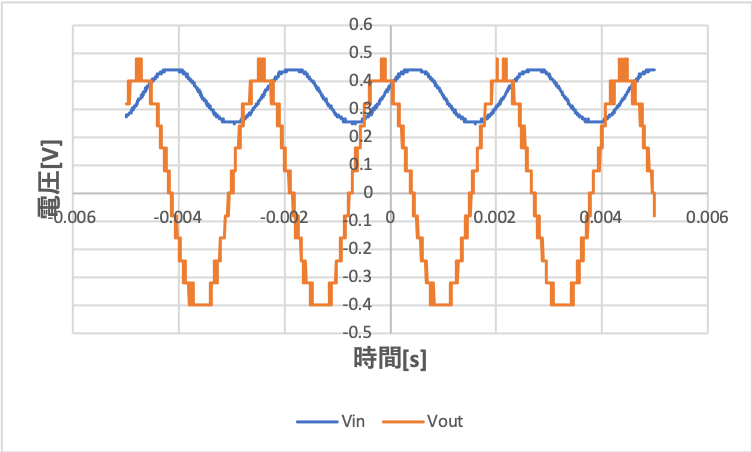
\includegraphics[width=0.8\linewidth]{fig54.png}
 \end{center}
 \caption{Band pass filter(Vin 5kHz)}
 \label{fig:54}
\end{figure}

\begin{figure}[htbp]
 \begin{center}
  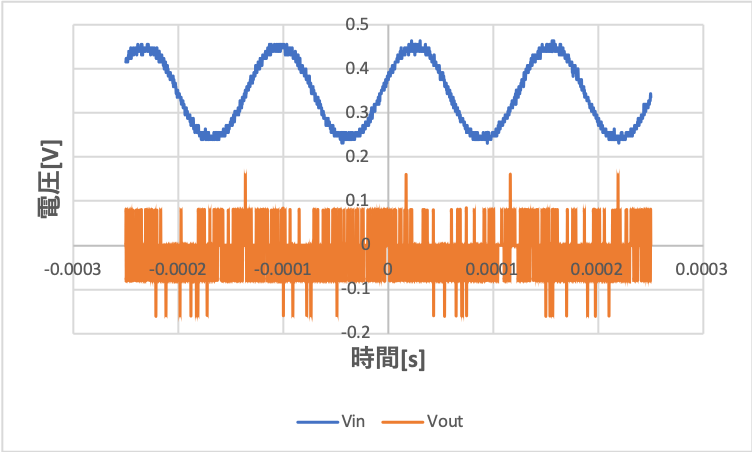
\includegraphics[width=0.8\linewidth]{fig55.png}
 \end{center}
 \caption{Band pass filter(Vin 10kHz)}
 \label{fig:55}
\end{figure}

\newpage


\documentclass[11pt, a4paper,twocolumn]{jarticle}
\usepackage[dvipdfmx]{graphicx}
\begin{document}

実験結果よりLow pass filterでは入力電圧の周波数が小さい時は元の矩形波を反転させた形の出力が得られたが,周波数が上がるにつれて元の矩形波が変化した際に遅れを生じるようになり指数関数的に追いつくような波形が得られた.
特に1kHzでの出力波は三角波のようになり,それ以上周波数が上がると出力は一定値となった.

また,High pass filterでは入力電圧の周波数が高くなるにつれて元の矩形を反転させたような出力が得られた.また低周波数領域では入力電圧が変化した瞬間だけ一瞬電圧の大きさがが大きくなりその後指数関数的に減少するような結果となった.

さらにBand pass filterでは10Hz付近では正弦波の重ね合わせのような出力が得られた.
これらの波の振幅は非常に小さかった.
また,100Hz付近になると入力の矩形波を反転させたような出力が得られた.
さらに周波数をあげると出力は一定値となった.

またそれぞれの場合において正弦波の入力を与えるとLow pass filterでは高周波数領域で振幅が小さくなり,High pass filterでは低周波数領域で振幅が小さくなり,Band pass filterでは低周波数領域と高周波数領域で振幅が小さくなった.
また総じてカットされる周波数での出力波は滑らかではなく不連続な波となった.

\subsubsection{Discussion}
今回はなぜ低周波数領域や高周波数領域の入力をカットできるのかを考察していく.
まず,図\ref{fig:13},図\ref{fig:14},図\ref{fig:15}における回路は前回の実験で行なった反転増幅回路とほぼ同じ構造をしているのがわかる.
そのことより今回の出力は入力を反転させたような波形であると予測できる.

Low pass filterについて考察を行う.
図\ref{fig:13}の回路においてキルヒホッフの法則を用いると以下の微分方程式を立てることができる.
\begin{equation}
    RC\frac{dV_{out}}{dt} + V_{out} = -V_{in}
\end{equation}

この微分方程式をとくと以下のような式を得る.
\begin{equation}
    V_{out} = -u(t)\left[1-exp\left(-\frac{t}{RC}\right)\right]
\end{equation}

この式よりtが十分大きい時expの部分は0に近づくため出力は入力の反転した値が出てくる.
一方で高周波の場合はexpは1に近づくので出力は0に近づいていくこととなり実験結果と一致することが確かめられた.

次にHigh pass filterについて考察を行う.
図\ref{fig:14}の回路においてキルヒホッフの法則を用いると以下の微分方程式を立てることができる.
\begin{equation}
    V_{out} = -RC\frac{d}{dt}(V_{out}+V_{in})
\end{equation}

この微分方程式をとくと以下のような式を得る.
\begin{equation}
    V_{out} = -u(t)exp\left(-\frac{t}{RC}\right)\
\end{equation}

この式よりtが十分小さい時expの値は1に近づくこととなり出力は入力の反転した値となる.
またtが十分大きい時はexpの値は0に近づくこととなり結果的に出力は0となる.
この性質は高周波数成分を通し,低周波数成分をカットする性質であるので実験の値とも一致することが確かめられた.

ここで得られた特定の周波数をカットするフィルターの応用例について考えてみる.
例えば,画像や音声において人間の目に見えないもしくは聞き取ることができない周波数成分はデータとして余計なのでフィルターに通してカットすることで,元のデータ量を落とすことができる.

\end{document}


%=============================================================
\newpage
\end{document}

\documentclass[11pt, a4paper,twocolumn]{jarticle}
\usepackage[dvipdfmx]{graphicx}
\usepackage{listings,jlisting}

\begin{document}
%=============================================================
\section{Measurement of the temperature dependence of the resistivity of $Bi_2Sr_2Ca_2Cu_3O_{10}$ as a superconductor($6^{th} day$)}

\subsection{Purpose}
超電導の転移温度の測定を通して超電導の原理について学ぶ.
\subsection{Procedure}
前回同様に図\ref{fig:29}のように温度依存性の測定のための実験装置を組み立てる.
次に超電導リボン($Bi_2Sr_2Ca_2Cu_3O_{10}$)の電圧-電流特性を四端子測定法で測定する.
この時超電導のヒステリシス特性を観察するために室温から超電導が起こる相転移温度まで下げていった場合と,超電導状態から室温に近づけていった場合の二パターンについて測定を行いそれぞれの結果を温度-抵抗値のグラフにプロットしていく.
測定の際は電流が100mAを超えないように注意して行う.

\subsection{Result}
測定の結果温度と抵抗値の関係をプロットすると以下のようなグラフが得られた.
ヒステリシスが測定され,室温から温度を下げていった場合よりも超電導状態から室温にあげていった時は結果が全体的に左にシフトした.
また実験結果より温度下降時は相転移温度は140Kほど,上昇時は130Kほどであることが確認された.

\begin{figure}[htbp]
 \begin{center}
  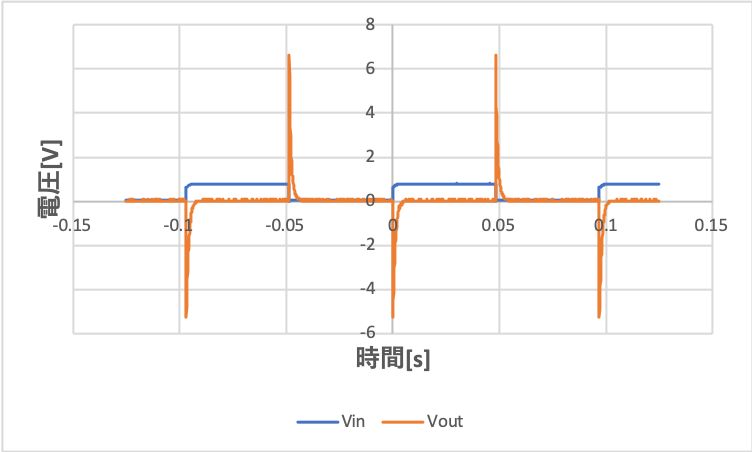
\includegraphics[width=0.8\linewidth]{fig39.png}
 \end{center}
 \caption{温度下降}
 \label{fig:39}
\end{figure}

\subsection{Discussion}
超電導が起こる理由について考える.
まず超電導が起きる極低温状態においては原子の熱振動は十分小さくなっていることが予想される.そこで一つの電子が原子に衝突すると原子が動かされ,プラスに帯電している原子は別の電子を引き寄せるという原理によって結果として電子同士が引き寄せられる現象が図\ref{fig:40}が起きる.
以上のようにして電子のペアについて片方が原子に衝突しても,その衝撃を片方がプラス,もう一方がマイナスに分散吸収してペア全体としては何事もなかったように進むことによって抵抗を感じずに電流を流すことができる.

次に超電導の応用について考える.
超電導状態では小さい電圧で多くの電流を流すことができるので非常に強い磁場を作り出すことが可能である.これはリニアモーターカーなどで利用される.
また量子コンピュータにおいては量子状態がノイズによって壊れることが問題であるためノイズを小さくするために超電導状態が用いられる.
もし超電導状態を室温で実現することができればリニアモータカーが新幹線よりもコストの低い乗り物になることができ,量子コンピュータの製作コストが格段に低くなることが予想される.

\begin{figure}[htbp]
 \begin{center}
  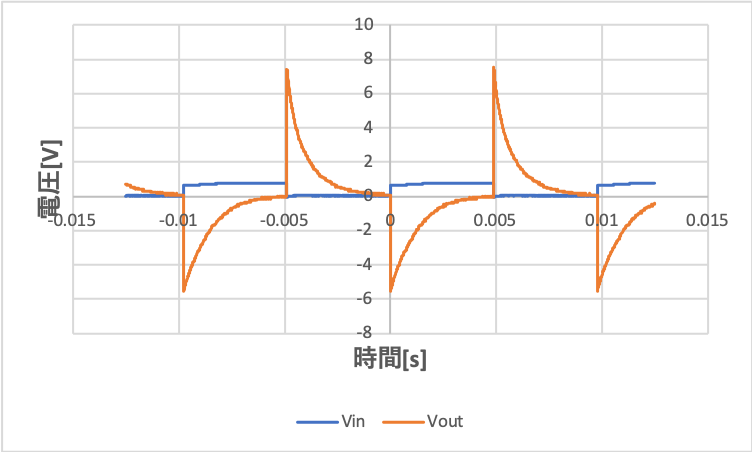
\includegraphics[width=0.8\linewidth]{fig40.png}
 \end{center}
 \caption{超電導メカニズム}
 \label{fig:40}
\end{figure}
%=============================================================
\newpage
\end{document}

%=============================================================
\end{document}
